%!TEX TS-program = xelatex
\documentclass[]{friggeri-cv}
\usepackage{afterpage}
\usepackage[]{hyperref}
\usepackage{smartdiagram}
% \usepackage[usenames, dvipsnames]{color}
\usepackage{xcolor}
\usepackage{enumitem}
\usepackage{multicol}




\setlist[itemize]{noitemsep, topsep=0pt}
\setlist[itemize]{leftmargin=*}

\hypersetup{
    pdftitle={},
    pdfauthor={},
    pdfsubject={},
    pdfkeywords={},
    colorlinks=false,       % no link border color
    allbordercolors=white,    % white border color for all
    hidelinks = true
}

\smartdiagramset{
    bubble center node font = \scriptsize,
    bubble node font = \scriptsize,
    % specifies the minimum size of the bubble center node
    bubble center node size = 0.01cm,
    %  specifies the minimum size of the bubbles
    bubble node size = 0.9cm,
    % specifies which is the distance among the bubble center node and the other bubbles
    distance center/other bubbles = 0.4cm,
    % sets the distance from the text to the border of the bubble center node
    distance text center bubble = 0.3cm,
    % set center bubble color
    bubble center node color = pblue,
    % define the list of colors usable in the diagram
    set color list = {lightgray, materialcyan, orange, green, materialorange, materialteal, materialamber, materialindigo, materialgreen, materiallime},
    % sets the opacity at which the bubbles are shown
    bubble fill opacity = 0.4,
    % sets the opacity at which the bubble text is shown
    bubble text opacity = 0.8,
}

\addbibresource{bibliography.bib}
\RequirePackage{xcolor}
\definecolor{pblue}{HTML}{0395DE}
% \definecolor{pblue}{HTML}{000080}


\begin{document}
\header{Landon}{ Wright}
      {Mechanical Engineer}

% Fake text to add separator
\fcolorbox{white}{gray}{\parbox{\dimexpr\textwidth-2\fboxsep-2\fboxrule}{
.....
}}
% In the aside, each new line forces a line break

\begin{aside}
	%\hfill \break
	\vspace{0.65 in}{~}
  \section{Telephone}
    (385) 312 2726
    ~
  \section{Mail}
    \href{mailto:landon.Wright91+resume@Gmail.com}{\textbf{Landon.Wright91@}\\gmail.com}
    ~
%   \section{Address}
%     815W 300S apt 1
%     Provo, UT 84601
%   \section{Git}
% %     \href{http://www.carminebenedetto.net}{carminebenedetto.net}
% %     \href{https://bitbucket.org/neoben}{bitbucket.org/neoben}
%     \href{https://github.com/landonbw}{github.com/landonbw}
  \section{Personal Skills}
    % 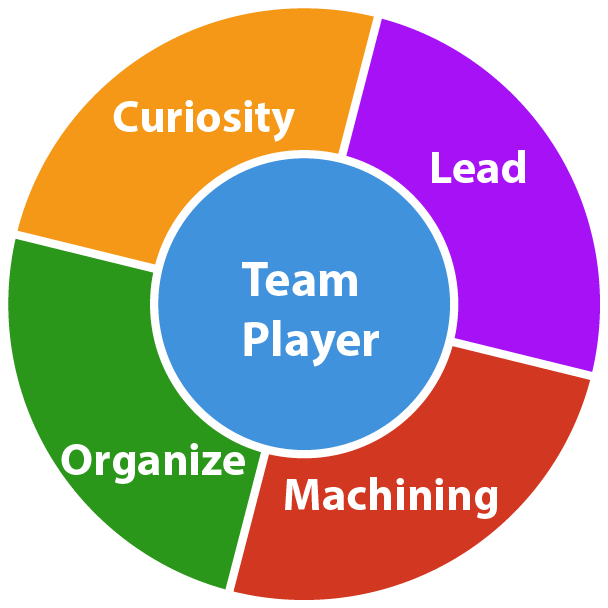
\includegraphics[width = 1.5in]{img/personalLandon.png}
%     % 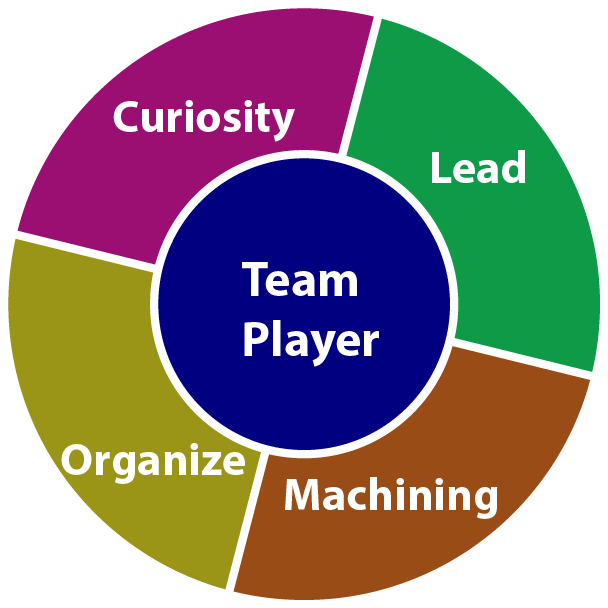
\includegraphics[width = 1.5in]{img/personalLandonDark.png}
    \smartdiagram[bubble diagram]{
        % \textbf{Team}\\\textbf{Player},
        % \textbf{Initiative},
        % \textbf{Curiosity},
        % \textbf{Problem}\\\textbf{Solving},
        % %\textbf{\vspace{2mm}Manage\vspace{2mm}},
        % \textbf{Manage},
        % \textbf{Organize}
        \textbf{Public}\\\textbf{Speaking},
        \textbf{Problem}\\\textbf{Solving},
        \textbf{Research},
        \textbf{Automation},
        \textbf{Leadership},
        \textbf{Hard}\\\textbf{Work}
    }
%     ~
    ~
    \section{CAD Knowledge}
    \textbf{NX}
\includegraphics[scale=0.40]{img/4stars.png}
    \textbf{Solidworks}
\includegraphics[scale=0.40]{img/3stars.png}
    \textbf{Inventor}
\includegraphics[scale=0.40]{img/3stars.png}
    \textbf{Fusion 360}
\includegraphics[scale=0.40]{img/3stars.png}
    \textbf{Catia}
\includegraphics[scale=0.40]{img/2stars.png}
    % \textbf{Creo}
\includegraphics[scale=0.40]{img/1stars.png}
    ~
    \section{Programming}
%    \vspace{1mm}
    % 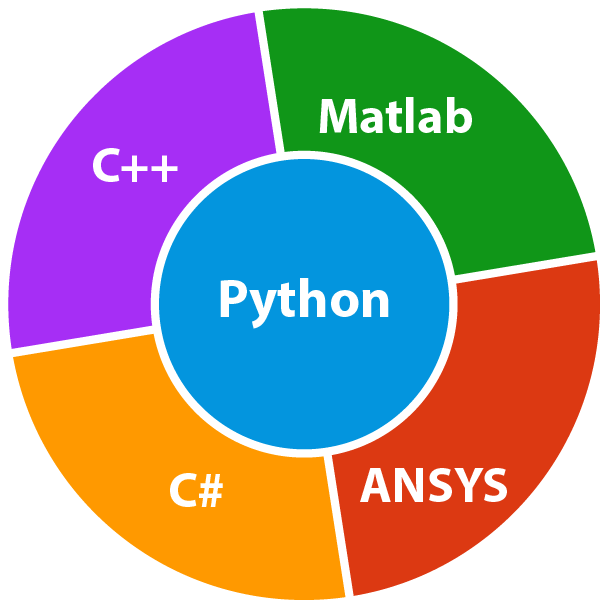
\includegraphics[width = 1.5in]{img/programmingLandon.png}
    % 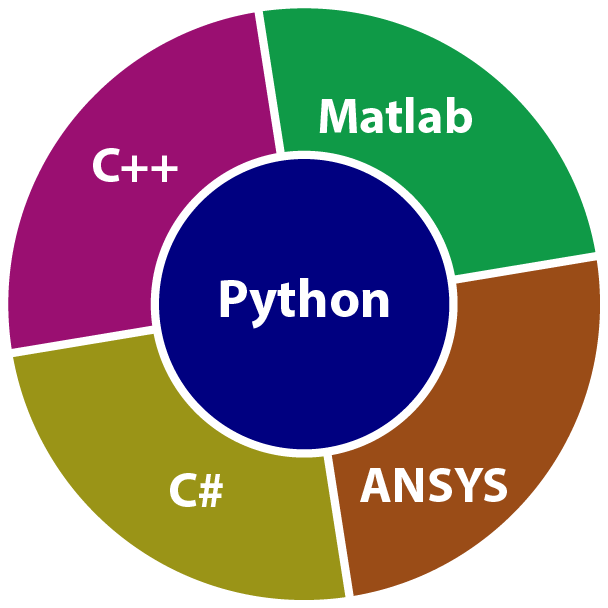
\includegraphics[width = 1.5in]{img/programmingLandonDark.png}
    \smartdiagram[bubble diagram]{
      \textbf{Python},
      \textbf{C/C++},
      \textbf{Matlab},
      \textbf{C\#},
      \textbf{ANSYS}\\\textbf{APDL},
      \textbf{Julia},
      \textbf{JSL\vspace{-4mm}}

      %\textbf{}
}
    ~
    \section{Languages}
    \textbf{English}
\includegraphics[scale=0.40]{img/5stars.png}
    \textbf{Spanish}
\includegraphics[scale=0.40]{img/3stars.png}
    ~
    \section{Certifications}
    Amateur Extra HAM
    GO PLM for NX
    ~
\end{aside}

\section{Education}
\vspace{-3mm}
\begin{entrylist}
    \entry
    {09/17 - 08/19}
    {Master of Science, Mechanical Engineering}
    {BYU, Provo UT}
    {GPA: 3.91\\Relevant Coursework: Systems Engineering and CAD Applications, Computer Aided Engineering Software Development, Optimization Techniques, Statistical Methods for Research}
    % {GPA: 3.91\\Relevant Coursework: Multi-Agent Systems, Statistical Methods for Research, Optimization Techniques, Systems Engineering and CAD Applications Computer Aided Engineering Software Development}

    \entry
    {01/12 - 04/17}
    {Bachelor of Science, Mechanical Engineering}
    {BYU, Provo UT}
    {GPA: 3.57}
    % {Relevant Coursework: Flight Dynamics and Control, Mechanical Systems Design Applications, Engineering Measurements}



\end{entrylist}

\vspace{-3.5mm}

\section{Skills and Abilities}
\vspace{-3mm}
\begin{entrylist}

    % \entry
    % {}
    % {Computer Aided Design (CAD)}
    % {}
    % {\vspace{-4mm}
    % \begin{itemize}
    %     % \item (Fusion) Recognized by Autodesk with two \$250 awards for excellence in part modeling
    %     % \item (Solidworks)  Created suite of parametric models to allow for rapid generation of customized parts to suit client needs
    %     \item (NX) Three years experience modeling aerospace components to evaluate performance of advanced CAD applications
    %     \item (Fusion/solidThinking Inspire) Designed, optimized and fabricated bike rack support mounts
    % \end{itemize}\vspace{1mm}}

    % \entry
    % {}
    % {Computer Aided Engineering}
    % {}
    % {\vspace{-4mm}
    % \begin{itemize}
    %     % \item Developed ANSYS models for static stress, large non-linear deflections, modal analysis, buckling and other failure modes
        
    %     % \item Experienced performing mathematical analysis in MathCAD and Maple
    %     \item Expertise creating complex parametric CAD models and assemblies in Solidworks and other packages
    %     \item Experienced with topology optimization for the developmen of maximally stiff parts with minimal weight
    %     \item Developed tools to automate swept part interferance detection in automotive applications
    % \end{itemize}}

    % \entry
    % {}
    % {Computer Programming}
    % {}
    % {\vspace{-4mm}
    % \begin{itemize}
    % \item (C\#) Contributed to development of over 50,000 lines of code interfacing with the NX API
    % % \item (C++)~Developed rope simulation software including dynamic force elongation and failure dynamics with integrated visualization
    % \item (Julia)~Created descrete event multi-agent simulation of autonomous vehicle networks to evaluate societal impacts of shared autonomous vehicles
    % % \item (Linux/C++)~Implemented iterative jacobi solver using multi-threading /processing techniques for use on high performance computing clusters
    % \item (Python) Created flight simulator, visualization system, and aircraft control systems for Micro Air Vehicles including PID control, total energy control, and Kalman filters and path planning algorithms
    % \item (Linux/Python/Sqlite)~Developed automated webscraping system to track, store, and provide notifications of classified ads.
    
    % \end{itemize}\vspace{1mm}}




    % \entry
    % {}
    % {Communication}
    % {}
    % {\vspace{-4mm}
    % \begin{itemize}
    % \item Awarded best new research for work presented at the 2017 International Technical Rescue Symposium
    % \item Presenter at the 2017 JMP Discovery Summit demonstrating statistical analysis of flight simulation statistics in JSL (Best presentation runner-up)
    % % \item Communicated with Peruvian residents and workers to successfully define requirements and design of adhesive free tea bag sealing device
    % % and oversaw progress towards achievement of technical and social constraints in development of products for tea packaging process in Peru
    % % \item Presented actionable results of academic research to volunteers and industry professionals at the 2017 International Technical Rescue Symposium
    
    % \end{itemize}\vspace{1mm}}

    % \entry
    % {}
    % {Test Development}
    % {}
    % {\vspace{-4mm}
    % \begin{itemize}
    %     \item Created qualification tests to verify acceptable performance of synthetic alternatives to natural pyrophyllite used in diamond production
    %     \item 
    % \end{itemize}
    % \vspace{1mm}}


    % \entry
    % {}
    % {Control Systems}
    % {}
    % {\vspace{-4mm}
    % \begin{itemize}
    %     \item (Python) Created flight simulator, visualization system, and aircraft control systems for Micro Air Vehicles including PID control, total energy control, and Kalman filters and path planning algorithms
    %     \item (Python) Implemented PID, State Space, and Loop Shaping control methods for a two rotor "Whirlybird"
    % \end{itemize}
    % \vspace{1mm}}




    \entry
    {}
    {Product Development}
    {}
    {\vspace{-4mm}
    \begin{itemize}
        \item Designed and constructed an adhesive free paper sealing device used to reduce tea bag packaging time by 85\%
        \item Recognized by Associate Administrator of National Nuclear Security Administration for excellence in design of nuclear ordinance tooling

        % \item Manufactured equipment to allow for the use of minimum quantity lubrication on an existing horizontal machining center
    \end{itemize}
    \vspace{1mm}}

    \entry
    {}
    {Statistical Analysis}
    {}
    {\vspace{-4mm}
    \begin{itemize}
    % \item (JMP) Determined which environmental factors have the largest impacts on webbing strength (Best new research ITRS 2017)
    \item (JMP) Co-presenter at 2017 JMP Discovery Summit (Best paper runner-up)
    \item Used Experimental design and statistical analysis principles to analyze environmental effects on webbing (Awarded Best New Research ITRS 2017)
    % \item Applied Design of Experiement knowledge to develop studies investigating environmental factors impacting strength of climbing webbing

    % \item (JMP) Analyzed statistical patterns in randomized experiments to determine factors that contribute to decreases in webbing breaking strength.
    %\item (JMP) Analyzed environmental factors that effect webbing strength in Search and Rescue applications -  Awarded best new research ITRS 2017
    % \item (Python/JMP) Predicted car values to within \$4000 through market tracking and analysis of over 100,000 car advertisements
    \end{itemize}\vspace{1mm}}




    \entry
    {}
    {Leadership}
    {}
    {\vspace{-4mm}
    \begin{itemize}
    \item Coordinated up to 10 students in verification testing of innovative multi-user CAD software
    % \item Team
    \item Led team of 3 students with \$50,000 budget to investigate CAD automation methods leading to a publication in CAD and Applications Journal
    % \item Prepared and presented project updates to multinational aerospace and automotive corporations to secure future funding for research activities
    % \item Led group of 12 students in modeling of wing structure for original Wright Flyer
    \end{itemize}\vspace{1mm}}




    % \entry
    % {}
    % {Research}
    % {}
    % {\vspace{-4mm}
    % \begin{itemize}
    % % \item Initiated novel research into development of a CAD model taxonomy
    % % \item Coordinated with corporate sponsors to obtain funding for research projects involving collaborative CAD tools
    % % \item Received corporate support for research regarding mechanical advantage of rappel devices
    % \item Received university funding to research and present the effect of environmental factors on the strength of climbing webbing
    % \item Awarded Best New Research at International Technical Rescue Symposium 2017
    % % \item Used JMP statistical package to analyze statistical effect of environmental factors on webbing strength
    % \end{itemize}\vspace{1mm}}



    % \entry
    % {}
    % {Prototype and Equipment Construction}
    % {}
    % {\vspace{-4mm}
    % \begin{itemize}
    % % \item Designed and constructed paper sealing device to improve productivity of a tea packaging factory in Peru
    % % \item Built and flew an RC aircraft in order to validate engineering calculations predicting flight characteristics
    % \item Manufactured equipment to allow for the use of minimum quantity lubrication on an existing horizontal machining center
    % \item Developed and built a testing apparatus in order to accurately measure the mechanical advantage of rappel devices
    % \item Constructed Large scale cutaway of a lock cylinder and key in order to teach elementary school students how locks and keys function together
    % % \item Oversaw design and construction of large scale kaleidoscope to support a university artist in the development of her final show for the Utah Museum of Contemporary Art.
    % \item Designed equipment to safely lift and transport nuclear ordnance of varying size.
    % \end{itemize}
    % \vspace{1mm}}




    % \entry
    % {}
    % {Finite Element Analysis}
    % {}
    % {\vspace{-4mm}
    % \begin{itemize}
    %     \item Created parametric models for analysis of various geometries and loading conditions in ANSYS
    %     \item Developed ANSYS models for static stress, large deflections, modal analysis, buckling and other failure modes
    % \end{itemize}
    % \vspace{1mm}}





\end{entrylist}

\vspace{-4mm}



\section{Experience}
\vspace{-3mm}
\begin{entrylist}

  \entry
    {8/19 - now}
    {Research and Development Engineer}
    {US Synthetic, Orem, UT}
    {\vspace{-4mm}
    \begin{itemize}
        \item Created standards to document and communicate learning in order to reduce redundant research efforts
        \item Developed methods to create increased pressure in polycrystalline diamond production
    \end{itemize}\vspace{1mm}}


  \entry
    {02/14 - 8/19}
    {Research Assistant}
    {BYU XDL, Provo, UT}
    {\vspace{-4mm}
    \begin{itemize}
        \item Developed agent based discrete event simulations of shared autonomous vehicles to identify optimal vehicle relocation algorithms
        % \item Planned and carried out user testing to evaluate the effectiveness of advanced and experimental CAD tools
        % \item Effectively planned and coordinated projects with research assistants and corporate sponsors to ensure exceptional performance on critical tasks and deadlines
        % \item Four years experience developing programmatic CAD automation tools for aerospace and automotive applications
        \item Co-founded Search and rescue arm of research leading to best new research award at the 2017 International Technical Rescue Symposium
        \item (C\#) Team lead of group developing algorithms to create simplified assembly representations for reduced CAD software load times
        % \item (Juila) Developed simulation to understand impacts of autonomous vehicles
        % \item (C\#) Developed and debugged multi-user collaborative CAD software
        % \item (C++/OpenCV) Designed tools to analyze mouse movement and error messages in screen recordings of user experiments
    \end{itemize}\vspace{1mm}}
    % {Worked with Boeing and other aerospace partners to secure funding, develop, and test collaborative CAD applications based in Siemens NX\\}
%   \entry
%     {04/16 - Now}
%     {Developer}
%     {BYU Cad Lab, Provo, UT}
%     {Contributed to development of advanced CAD components in C\#\\}
%   \entry
%     {02/14 - 04/16}
%     {Tester Lead}
%     {BYU Cad Lab, Provo, UT}
%     {Organized testing team in performance validation of revolutionary multi-user CAD package (NX-based)\\}
%   \entry
%     {04/16 - 09/16}
%     {Research Assistant}
%     {Compliant Mechanisms Research Laboratory, Provo, UT}
%     {\vspace{-4mm}
%     \begin{itemize}
%         \item Implemented technology push product design methods to discover novel applications of origami inspired compliant mechanisms
%         \item Created a process to manufacture textiles with shape memory
%     \end{itemize}\vspace{1mm}}
    % {Investigated possible techniques to apply origami inspired compliant mechanisms to manufacturing processes\\}

\entry
    {05/18 - 08/18}
    {Systems Engineer Intern}
    {Honeywell, Phoenix, AZ}
    {\vspace{-4mm}
    \begin{itemize}
        % \item Developed automation toolkit for Simulink simulations resulting in a 90\% reduction in analysis time and enabling monte carlo analyses previously considered to be infeasible
        \item Developed automation toolkit simulations resulting in a 90\% reduction in analysis time
        % \item (MATLAB) Reduced circuit analysis time from three days to three hours with a 98\% reduction in rework time through programmatic automation
        % \item Eliminated redundant test methods by evaluating and comparing competing requirements of RTCA DO-160, MIL-STD-810, and MIL-STD-461
        \item Prepared and presented critical design review slides to customer

    \end{itemize}\vspace{1mm}}

  \entry
    {04/15 - 09/15}
    {Engineering Intern}
    {Precorp Inc, Spanish Fork, UT}
    {\vspace{-4mm}
    \begin{itemize}
        % \item Analyzed function and purpose of pyrophyllite in synthetic diamond production in order to propose materials with an annual cost saving of \$100,000
        % \item Generated a cost savings of \$100,000 annually by evaluating synthetic alternatives to pyrophyllite in poly-crystalline diamond production
        \item Developed qualification tests for the evaluation of synthetic alternatives to natural pyrophyllite
        % \item Investigated methods of non-destructive crack detection in poly-crystalline diamond to eliminate time intensive manual inspection
        \item Measured and quantified factory throughput to enable verifiable lean improvements
     \end{itemize}\vspace{1mm}}
    % {Improved manufacturing and inspection techniques for polycrystalline diamond cutting tools used in the aerospace and automotive industries}
    % \entry
    % {Ongoing}
    % {Personal Projects}
    % {Projects completed while student at BYU}
    % {\vspace{-4mm}
    % \begin{itemize}
    %     \item Initiated, obtained funding, carried out, and presented research on the impact of environmental factors on climbing webbing strength
    %     \item Designing computer vision based CNC honey dispensing device
    %     \item (Fusion/solidThinking Inspire) Designed, optimized and fabricated bike rack support mounts

    % \end{itemize}\vspace{1mm}}
\end{entrylist}

\vspace{-4mm}








% \section{Awards}
% \vspace{-5mm}
% \begin{multicols}{2}
%     \begin{itemize}
%         \item Capstone project recognized as outstanding design by the National Nuclear Security Administration
%         \item Best new research ITRS 2017
%     \columnbreak
%         \item thing 2
%     \end{itemize}
% \end{multicols}
% ~
~
\end{document}
